\documentclass[tikz,border=10pt]{standalone}
\usepackage{helvet}
\renewcommand{\familydefault}{\sfdefault}
\usepackage{pgfplots}
\pgfplotsset{compat=1.18}
\usepgfplotslibrary{fillbetween}

\definecolor{emeraldpine}{HTML}{1A4D3E}
\definecolor{harvardcrimson}{HTML}{A51C30}
\definecolor{ethdarkblue}{HTML}{1F407A}
\definecolor{ethpetrol}{HTML}{007A87}
\definecolor{ethbronze}{HTML}{B87333}
\definecolor{ink}{HTML}{1A202C}
\definecolor{cardbg}{HTML}{F8FAFC}

\begin{document}
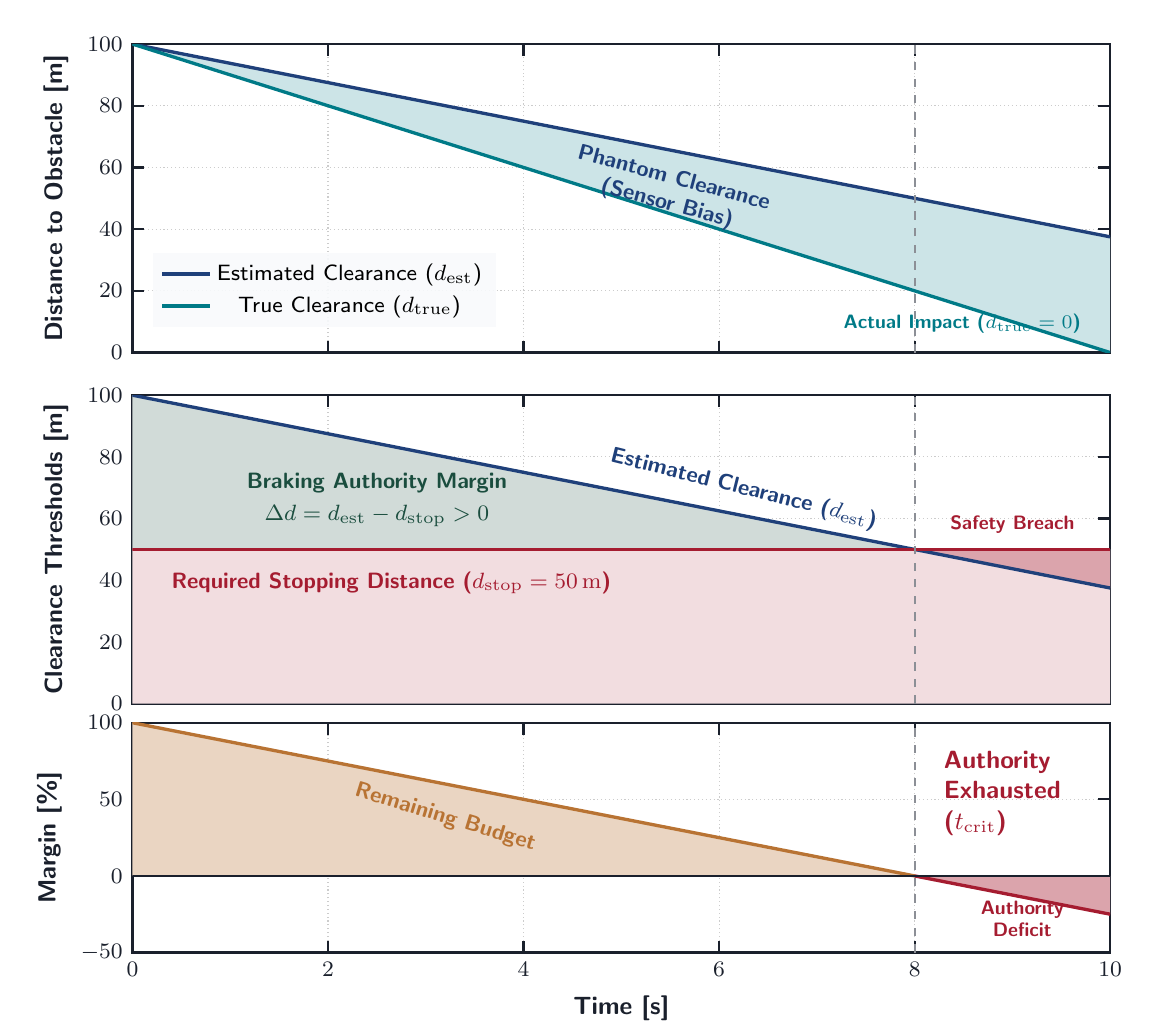
\begin{tikzpicture}

% Shared Axis parameters
\pgfplotsset{
    every axis/.append style={
        width=14cm,
        axis line style={ink, thick},
        tick style={ink, thick},
        tick label style={ink, font=\footnotesize},
        label style={ink, font=\small\bfseries},
        grid=major,
        grid style={densely dotted, black!20},
        xmin=0, xmax=10,
        xtick={0,2,4,6,8,10},
    }
}

% Top Panel: Distances
\begin{axis}[
    name=top,
    height=5.5cm,
    ymin=0, ymax=100,
    ytick={0,20,40,60,80,100},
    ylabel={Distance to Obstacle [m]},
    xticklabels={\empty},
    legend style={at={(0.02,0.08)}, anchor=south west, font=\footnotesize, draw=none, fill=cardbg, fill opacity=0.9, text opacity=1, nodes={inner sep=2pt}},
]

\addplot[name path=est, ethdarkblue, very thick, domain=0:10] {100 - 6.25*x};
\addlegendentry{Estimated Clearance ($d_{\mathrm{est}}$)}

\addplot[name path=true, ethpetrol, very thick, domain=0:10] {100 - 10*x};
\addlegendentry{True Clearance ($d_{\mathrm{true}}$)}

\addplot[ethpetrol!20] fill between[of=true and est];
\node[ethdarkblue, font=\footnotesize\bfseries, align=center, rotate=-15] at (axis cs: 5.5, 52) {Phantom Clearance\\(Sensor Bias)};

\draw[dashed, ink!50, thick] (8,0) -- (8,100);
\node[ethpetrol, font=\scriptsize\bfseries, anchor=south east] at (axis cs: 9.8, 3) {Actual Impact ($d_{\mathrm{true}}=0$)};

\end{axis}

% Middle Panel: Braking Margin
\begin{axis}[
    name=mid,
    at={(top.below south west)},
    anchor=north west,
    yshift=-0.3cm,
    height=5.5cm,
    ymin=0, ymax=100,
    ytick={0,20,40,60,80,100},
    ylabel={Clearance Thresholds [m]},
    xticklabels={\empty},
]

\addplot[name path=est2, ethdarkblue, very thick, domain=0:10] {100 - 6.25*x};
\addplot[name path=stop, harvardcrimson, very thick, domain=0:10] {50};
\addplot[name path=zero2, draw=none, domain=0:10] {0};

% Danger zone
\addplot[harvardcrimson!15] fill between[of=zero2 and stop];

% Safe margin
\addplot[emeraldpine!20] fill between[of=stop and est2, soft clip={domain=0:8}];

% Negative margin (phantom safety)
\addplot[harvardcrimson!40] fill between[of=est2 and stop, soft clip={domain=8:10}];

% Non-colliding labels
\node[ethdarkblue, font=\footnotesize\bfseries, rotate=-14, anchor=south] at (axis cs: 6.2, 63) {Estimated Clearance ($d_{\mathrm{est}}$)};
\node[harvardcrimson, font=\footnotesize\bfseries, anchor=north west] at (axis cs: 0.3, 46) {Required Stopping Distance ($d_{\mathrm{stop}} = 50\,\mathrm{m}$)};

\node[emeraldpine, font=\footnotesize\bfseries, align=center] at (axis cs: 2.5, 66) {Braking Authority Margin\\[2pt]$\Delta d = d_{\mathrm{est}} - d_{\mathrm{stop}} > 0$};

\draw[dashed, ink!50, thick] (8,0) -- (8,100);
\node[harvardcrimson, font=\scriptsize\bfseries, anchor=south] at (axis cs: 9.0, 52) {Safety Breach};

\end{axis}

% Bottom Panel: Margin Percentage
\begin{axis}[
    name=bot,
    at={(mid.below south west)},
    anchor=north west,
    yshift=-0.3cm,
    height=4.5cm,
    ymin=-50, ymax=100,
    ytick={-50, 0, 50, 100},
    ylabel={Margin [\%]},
    xlabel={Time [s]},
]

\addplot[name path=perc, draw=none, domain=0:10] {100 - 12.5*x};
\addplot[name path=zero3, draw=none, domain=0:10] {0};

\addplot[ethbronze!30] fill between[of=zero3 and perc, soft clip={domain=0:8}];
\addplot[harvardcrimson!40] fill between[of=zero3 and perc, soft clip={domain=8:10}];

\addplot[ethbronze, very thick, domain=0:8] {100 - 12.5*x};
\addplot[harvardcrimson, very thick, domain=8:10] {100 - 12.5*x};
\addplot[ink, thick] coordinates {(0,0) (10,0)};

\draw[dashed, ink!50, thick] (8,-50) -- (8,100);
\node[harvardcrimson, font=\small\bfseries, anchor=south west, align=left] at (axis cs: 8.2, 20) {Authority\\Exhausted\\($t_{\mathrm{crit}}$)};

\node[ethbronze, font=\footnotesize\bfseries, rotate=-17] at (axis cs: 3.2, 38) {Remaining Budget};
\node[harvardcrimson, font=\scriptsize\bfseries, align=center] at (axis cs: 9.1, -28) {Authority\\Deficit};

\end{axis}

\end{tikzpicture}
\end{document}
